Now we define the dual forms of the $\mathbb{R}$-vector space $V$ and the basis $\alpha_i$ as

\begin{equation}
 V^* := \{f: V \mapsto \mathbb{R}\  \text{linear} \}
\end{equation}
and

\begin{equation}
  \alpha_i^* (\alpha_j) := \delta_{ij}
\end{equation}

We also define a new mapping $\sigma^*$

\begin{equation}
 \sigma^* : W \mapsto GL(V^*)
\end{equation}
which is also an injective homomorphism. This function can also be defined as $\sigma^*(w) := \sigma(w^{-1})^T$, which means that if $f \in V^*$, then $\sigma^*(w)(f) = \sigma(w^{-1})^T(f) = f \circ \sigma(w^{-1})$.

We also define a natural pairing on $V^* \cross V$:

\begin{equation}
  (f,v) := f(v) \in \mathbb{R}
\end{equation}

This pairing can be developed as such:

\begin{equation}
(wf, wv) = (\sigma^*(w)(f), \sigma(w)(v)) = (f,v)
\end{equation}

We proceed to define some hyperplanes based on the dual forms of the objects that we have been using until now.

\begin{definition}
  For every $s_i \in S$ we have the following hyperplanes:

  \begin{equation}
    H_{s_i} := \{f \in V^* |\ (f, \alpha_i) = 0\}
  \end{equation}

  \begin{equation}
    A_{s_i} := \{f \in V^* |\ (f, \alpha_i) > 0\}
  \end{equation}

\end{definition}

We can define the \emph{fundamental chamber} $C$ as the intersection of the $A_{s_i}$ hyperplanes for every $s_i \in S$ and $D = \bar{C}$ its closure. Given $I \subseteq S$, we can also define $C_I := (\cap_{s\in I} H_s \cap (\cap_{s\in I} A_s))$.

\begin{figure}
  \begin{center}
\begin{tikzpicture}

	% general shift to north east
	\draw[semithick] (0,-2.5) -- (0,2.5);% center line
	\draw[->, semithick] (0,0) -- (1.3,0);% horizontal line
  \draw[<-, semithick] (-0.5,0.8) -- (0,0);% first symmetry
  \draw[semithick] (2.16,1.25) -- (-2.16,-1.25);% second symmetry

  % axis
  \def\offAx{0.2}
  \draw (-0.65,1) node {$\alpha_2$};
  \draw (1.5,0) node {$\alpha_1$};
  \draw (2.16+\offAx+0.1,-1.25-\offAx) node {};
  \draw (2.16+\offAx+0.1,+1.25+\offAx-0.1) node {$H_{s_2}$};
  \draw (0,2.7) node {$H_{s_1}$};


\end{tikzpicture}
\end{center}
\caption{The representative hyperplanes for $S_3$. In red is the hyperplane $A_{s_1}$ and in blue is the hyperplane $A_{s_2}$. Their intersection is $C$ (if you add the lines of $H_{s_1}$ and $H_{s_2}$ it is indeed its closure $\bar{C}$). -> remarque, j'arrive pas à dessiner les regions, faudra voir comment ça marche ...}
\label{fig:hyper}
\end{figure}

\begin{example}
    We proceed to visualize these hyperplanes on the plane for the coxeter group \dynkin[labels={s_1,s_2},label macro/.code={#1}]{A}{2} with a label of $s_3$.
\end{example}


We also define some more a Tits cone:

\begin{equation}
  U:= \cup_{w\in W} w (D)
\end{equation}

and

\begin{equation}
  \zeta := \{w(C_I)|\ w\in W, I \subseteq S\}
\end{equation}

\begin{theorem}
  \label{theo:stabilizer}
Let $w \in W$ and $I,J \subseteq S$
  \begin{itemize}
    \item (a) If $w (C_I) \cap C_J = \emptyset$, then $I = J$ and $w(C_I) = C_I$. Moreover $W_I$ is the stabilizer of $C_I$ and $\zeta$ is a partition of $U$ and $w \in W_I$.
    \item (b) $D$ is a fundamental domain for action of $w$ in $U$: the $W$-orbit of each point of $U$ meets $D$ in exactly one point.
    \item (c) $U$ is a convex cone, and every closed line segment in $U$ meets finitely many elements of $\zeta$
  \end{itemize}
\end{theorem}

\begin{example}
  Draw things of the blackboard
\end{example}

\begin{remark}
  Every element of $W_I$ fixes every point of $C_I$. Conversely, if $s \in S$ fixes a point $f \in C_I$, then with $s\in I$:

  \begin{equation}
    (f,\alpha_s) = (sf, s\alpha_s) = (f, -\alpha_s) = -(f,\alpha_s)
  \end{equation}

  so $(f,\alpha_s) = 0$, which means that $f \in H_s$.
\end{remark}

\begin{lemma}
  Let $s \in S$ and $w \in W$. Then $l(sw) > l(w)$ if and only if $w(C) \subseteq A_s$. Also, $l(sw) < l(w)$ if and only if $w(C) \subseteq -A_s$
\end{lemma}

\begin{proof}
  We have that $l(sw) > l(w)$ if and only if $l(w^{-1}) > l(w^{-1})$ and equivalently, by theorem, if and only if $w^{-1}\alpha_s > 0$.

  If $f \in C$, then $(wf, \alpha_s) > 0$ if and only if $(f, w^{-1}(\alpha_s)) > 0$. So $(f, w^{-1}(\alpha_s)) > 0$ for all $f \in C$ if and only if $w^{-1}(\alpha_s) > 0$. Which means that $w(C) \subseteq A$ if and only if $l(sw) > l(w)$.
\end{proof}

With this first results, we proceed to prove theorem \ref{theo:stabilizer}.

\begin{proof}
  First we prove (a) by induction on $l(w)$:\\

  If $l(w) = 0$, then $I$ and $J$ are the same sets.

  If $l(w) > 0$, let $s \in S$ be such that $l(sw) < l(w)$. So $l(s(sw)) > l(sw)$. We know by the last lemma that $sw(C) \subseteq A_s$, so $w(C) \subseteq sA_s = -A_s$. By continuity, $w(D) = w(\bar{C}) \subseteq \bar{-A_s} = -A_s \cup H_s$. Since $D \subseteq \bar{A_s}$, then we have $D\cap w(D) \subseteq H_s$. But $C_J \subseteq D$ and $w(C_I) \subseteq w(D)$, so $w(C_I) \cap C_J \subseteq H_s$. Since $w(C_I) \cap C_J \neq \emptyset$, there exists some point $p \in w(C_I) \cap C_J \subseteq C_J$ fixed by $s$.

  So $s \in J$ which gives us:

  \begin{equation}
    \begin{split}
      C_J\cap sw(C_I) = sC_J \cap sw)(C_I) = s(C_J \cap w(C_I)) \neq \emptyset
    \end{split}
  \end{equation}

  By induction, $I = J$ and $sw \in W_i$, so we also have $w \in W_I$ and $s \in J = I$ which means also that $sw(C_I) = C_I$, then $w(C_I) = C_I$. So the sets $w(C_I)$ are disjoint as $w$ rows in the left coxeter representation of $W_I$ and $I \subseteq S$. \qed\\


  Next, we prove (b).
  Suppose that $f,g \in D$, $w\in W$ such that $w(f) = g$. Say $f \in C_I$ and $g \in C_J$ so that $w(C_I) \cap C_J \neq \emptyset$.

  By (a), $I = J$ and $w \in W_I$, so $f = w(f) = g$. \qed\\

  Finally, we prove (c). In this proof it is enough to show that a closed line segment $[f,g]$ where $f,g \in U$ is covered by finitely elements of $\zeta$. If $f,g \in D$ then this is clear. Say $f \in D, g \in w(D)$., we have then $[f,g] \cap D = [f,h]$, so $h \in D \setminus C$. We finally have to discuss the same for $[h,g]$. We proceed by induction:

  Let $l(w) > 0$:

  \begin{equation}
    I := \{s \in S|\ g \in -A_s\} \neq \emptyset
  \end{equation}

For some $s \in I$, we must have $h \in H_s$, since $g \in -A_s$, we must have $w(D) \subseteq \bar{-A_s}$. By the lemma, $l(sw) < l(w)$.

By induction applied to $h\in D$ and $s(g) \in sw(D)$, $[h,s(g)]$ is covered by finitely many elements in $\zeta$. Applying $s$, we get the covering for $[h,g]$. \qed
\end{proof}

\subsection{Coxeter complexes}

\begin{definition}
  A \emph{simplicial complex} on a set $S$ is a collection of subsets $\zeta$ of $S$ such that:
  \begin{enumerate}
    \item $\emptyset \in \zeta$
    \item $A \in \zeta$ and $B \subseteq A$, then $B \in \zeta$.
  \end{enumerate}
\end{definition}

The ``vertices" are the cosets of maximal parabolic subgroups. A finite set of vertices is a simplex is their intersection is non-empty.


\begin{figure}
  \begin{center}
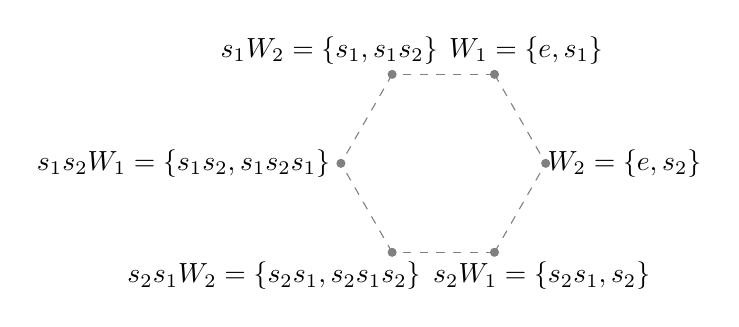
\begin{tikzpicture}
  \def\offX{0.65}
  \def\offY{1.13}
	\draw[dashed,color=gray] (0+\offX,0+\offY) -- (0.65+\offX,-1.13+\offY);% e to s_1
  \draw[dashed,color=gray] (0+\offX,0-\offY) -- (0.65+\offX,-1.13+\offY);% e to s_2
	\draw[dashed,color=gray] (0+\offX,0+\offY) -- (0-\offX,0+\offY);% s_1 to s_1s_2
  \draw[dashed,color=gray] (0+\offX,0-\offY) -- (0-\offX,0-\offY);% s_2 to s_2s_1
  \draw[dashed,color=gray] (0-\offX,0+\offY) -- (-1.3,0);% s_1s_2 to s_1s_2s_1
  \draw[dashed,color=gray] (0-\offX,0-\offY) -- (-1.3,0);% s_2s_1 to s_2s_1s_2

  \draw [fill=gray, color=gray](1.3,0) circle (0.05);
  \draw [fill=gray, color=gray](-1.3,0) circle (0.05);
  \draw [fill=gray, color=gray](0+\offX,0+\offY) circle (0.05);
  \draw [fill=gray, color=gray](0-\offX,0+\offY) circle (0.05);
  \draw [fill=gray, color=gray](0+\offX,0-\offY) circle (0.05);
  \draw [fill=gray, color=gray](0-\offX,0-\offY) circle (0.05); % s_1s_2

  \draw (2.3,0) node {$W_2 = \{e,s_2\}$};
  \draw (-3.3,0) node {$s_1s_2W_1 = \{s_1s_2,s_1s_2s_1\}$};
  \draw (0+\offX + 0.40,0+\offY + 0.30) node {$W_1 = \{e,s_1\}$};
  \draw (0+\offX + 0.60,0-\offY - 0.30) node {$s_2W_1 = \{s_2s_1,s_2\}$};
  \draw (0-\offX - 0.80,0+\offY + 0.30) node {$s_1W_2 = \{s_1,s_1s_2\}$};
  \draw (0-\offX - 1.5,0-\offY - 0.30) node {$s_2s_1W_2 = \{s_2s_1,s_2s_1s_2\}$};
\end{tikzpicture}
\end{center}
\caption{A simplicial complex.}
\label{fig:simplicial}
\end{figure}

\begin{example}
  For the sets $W_1 = W_{s_1} = {e,s_1}$ and $W_2 = W_{s_2} = {e,s_2}$ we have in figure \ref{fig:simplicial} the representation of its simplicial complex. You may notice that the nodes are adjacent if they have an element in common.
\end{example}
